
%% Based on a TeXnicCenter-Template by Tino Weinkauf.
%%%%%%%%%%%%%%%%%%%%%%%%%%%%%%%%%%%%%%%%%%%%%%%%%%%%%%%%%%%%%

%%%%%%%%%%%%%%%%%%%%%%%%%%%%%%%%%%%%%%%%%%%%%%%%%%%%%%%%%%%%%
%% HEADER
%%%%%%%%%%%%%%%%%%%%%%%%%%%%%%%%%%%%%%%%%%%%%%%%%%%%%%%%%%%%%
%\documentclass[onecolumn, 11pt, conference, compsocconf]{IEEEtran}
\documentclass[onecolumn, 12pt, article]{IEEEtran}
\usepackage{times,color,amsmath,amssymb,amsthm,comment,graphicx,cite,multirow}
%\documentclass[letterpaper,oneside,11pt]{letter}
% Alternative Options:
%	Paper Size: a4paper / a5paper / b5paper / letterpaper / legalpaper / executivepaper
% Duplex: oneside / twoside
% Base Font Size: 10pt / 11pt / 12pt


%% Language %%%%%%%%%%%%%%%%%%%%%%%%%%%%%%%%%%%%%%%%%%%%%%%%%
\usepackage[USenglish]{babel} %francais, polish, spanish, ...
\usepackage[T1]{fontenc}
\usepackage[ansinew]{inputenc}

\usepackage{lmodern} %Type1-font for non-english texts and characters
\usepackage{algorithm}
\usepackage{algpseudocode}
\usepackage{float}

%% Packages for Graphics & Figures %%%%%%%%%%%%%%%%%%%%%%%%%%
%\usepackage{graphicx} %%For loading graphic files
%\usepackage{subfig} %%Subfigures inside a figure
%\usepackage{tikz} %%Generate vector graphics from within LaTeX

%% Please note:
%% Images can be included using \includegraphics{filename}
%% resp. using the dialog in the Insert menu.
%% 
%% The mode "LaTeX => PDF" allows the following formats:
%%   .jpg  .png  .pdf  .mps
%% 
%% The modes "LaTeX => DVI", "LaTeX => PS" und "LaTeX => PS => PDF"
%% allow the following formats:
%%   .eps  .ps  .bmp  .pict  .pntg


%% Math Packages %%%%%%%%%%%%%%%%%%%%%%%%%%%%%%%%%%%%%%%%%%%%
\usepackage{amsmath}
\usepackage{amsthm}
\usepackage{amsfonts}
\usepackage{amssymb}
%\usepackage{array,MnSymbol}


%% Line Spacing %%%%%%%%%%%%%%%%%%%%%%%%%%%%%%%%%%%%%%%%%%%%%
\usepackage{setspace}
\singlespacing        %% 1-spacing (default)
%\onehalfspacing       %% 1,5-spacing
%\doublespacing        %% 2-spacing


%% Other Packages %%%%%%%%%%%%%%%%%%%%%%%%%%%%%%%%%%%%%%%%%%%
%\usepackage{a4wide} %%Smaller margins = more text per page.
\usepackage{fancyhdr} %%Fancy headings
\usepackage{listings}
\usepackage{capt-of}


%
% Theorem like environments
%
\newtheorem{problem}{Problem}%
%\numberwithin{problem}{section}
\newtheorem{theorem}{Theorem}%
\newtheorem{acknowledgment}{Acknowledgment}%
%\newtheorem{algorithm}{Algorithm}%
\newtheorem{assumption}{Assumption}%
\newtheorem{axiom}{Axiom}%
\newtheorem{case}{Case}%
\numberwithin{case}{problem}
\newtheorem{claim}{Claim}%
\newtheorem{conclusion}{Conclusion}
\newtheorem{condition}{Condition}
\numberwithin{condition}{problem}
\numberwithin{condition}{subsection}
\newtheorem{conjecture}{Conjecture}
\newtheorem{corollary}{Corollary}
\newtheorem{criterion}{Criterion}
\newtheorem{definition}{Definition}
\numberwithin{definition}{section}
\newtheorem{example}{Example}
\newtheorem{exercise}{Exercise}%
\newtheorem{lemma}{Lemma}%
\newtheorem{notation}{Notation}%
\theoremstyle{remark}
\newtheorem{question}{Question}%
\numberwithin{question}{problem}
\theoremstyle{plain}
\newtheorem{answer}{Answer}%
\numberwithin{answer}{problem}
\newtheorem{proposition}{Proposition}%
\newtheorem{remark}{Remark}%
\newtheorem{solution}{Solution}%
\numberwithin{solution}{section}
\newtheorem{summary}{Summary}%
\numberwithin{equation}{section}%
\newtheorem{option}{Option}



\raggedbottom
%%%%%%%%%%%%%%%%%%%%%%%%%%%%%%%%%%%%%%%%%%%%%%%%%%%%%%%%%%%%%
%% Remarks
%%%%%%%%%%%%%%%%%%%%%%%%%%%%%%%%%%%%%%%%%%%%%%%%%%%%%%%%%%%%%
%
% Note:
% 1. Edit the used packages and their options (see above).
% 2. If you want, add a BibTeX-File to the project
%    (e.g., 'literature.bib').
% 3. Happy TeXing!
%
%%%%%%%%%%%%%%%%%%%%%%%%%%%%%%%%%%%%%%%%%%%%%%%%%%%%%%%%%%%%%

%%%%%%%%%%%%%%%%%%%%%%%%%%%%%%%%%%%%%%%%%%%%%%%%%%%%%%%%%%%%%
%% Options / Modifications
%%%%%%%%%%%%%%%%%%%%%%%%%%%%%%%%%%%%%%%%%%%%%%%%%%%%%%%%%%%%%

%\input{options} %You need a file 'options.tex' for this
%% ==> TeXnicCenter supplies some possible option files
%% ==> with its-templates (File | New from Template...).





%% BEGIN DOCUMENT
\begin{document}

%% Title Page
\title{Java Sorting Algorithms Comparison}
\author{Preston Stosur-Bassett}
\date{February 23, 2015}
\maketitle

\pagestyle{fancy}
\fancyhead[R]{Java Sorting Algorithms Run-Time Analysis, page \thepage}
\fancyhead[L]{Preston Stosur-Bassett}

%% BEGIN ABSTRACT
\begin{abstract}

%% END ABSTRACT
\end{abstract}

%% BEGIN MOTIVATION
\section{Motivation}
In order to show how an algorithm might run on a given set of hardware, and how the algorithm will perform when given large amounts of data, algorithms are analysed. Sorting algorithms sort data into a natural order. By analysing sorting algorithms, the fastest algorithm for a given problem can be determined. 
%% END MOTIVATION

%% BEGIN BACKGROUND
\section{Background}
A sorting algorithm is used to sort data with a natural order. One such sorting algorithm is insertion sort, which sorts by iterating through a list of data, taking the current position, and repositioning it into a more appropriate place in the list. Heap sort is another sorting algorithm that greatly differs than insertion sort in that it uses a divide, conquer, and combine method; meaning that it breaks the set it is sorting into subsets until the subsets can no longer be broken up and then merge sort combines the subsets together rendering the correct answer. %% Write this for heap sort. 
%% END BACKGROUND

%% BEGIN PROCEDURE
\section{Procedure}
An insertion sort can be implemented in a multitude of languages using the pseudocode provided in Algorithm 1.
\newline
\textbf{Insertion Sort Pre-Condition}: A is a non-empty array of data with a natural order.
\newline
\textbf{Insertion Sort Post-Condition}: A' is a permutation of A (containing all the same elements) in strictly non-decreasing order.
\begin{algorithm}
\caption {\textsc{Insertion-Sort}(A)}
\label{algo:insertionsort}
\begin{algorithmic}[1]
\Procedure{Insertion-Sort}{A}
\If{$A.length < 2$}
\State{\Return{$A$}}
\EndIf
\State{$i = 2$}
\While{$i$ upto $A.length$}
	\State{$key = A[i]$}
	\State{$j = i - 1$}
	\While{$j$ downto $1$ and $key < A[j]$}
		\State{$A[j + 1] = A[j]$}
		\State{$j = j - 1$}
	\EndWhile
	\State{$A[j+1] = key$}
	\State{$i = i + 1$}
\EndWhile
\State{\Return{$A$}}
\EndProcedure
\end{algorithmic}
\end{algorithm}
\newline
\textbf{Insertion Sort Outer-Loop Invariant}: The subarray A'[1 ... i - 1] contains all the same elements as the subarray A[1 ... i - 1].
\newline 
\textbf{Insertion Sort Outer-Loop Initialization}: The outer-loop invariant holds because A'[1 ... i - 1] and A[1 ... i - 1] both contain the same one element.
\newline
\textbf{Insertion Sort Outer-Loop Maintenance}: The outer-loop invariant holds because A'[1 ... i - 1] and A[1 ... i - 1] both contain the same elements, although they may be in different orders.
\newline
\textbf{Insertion Sort Outer-Loop Termination}: When the outer-loop terminates, i = A.length, which implies that the entire array has been traversed and the guard has been negated. The negation of the guard implies that A'[1 ... i - 1] contains all the elements in A[1 ... i - 1].
\newline
\newline
\textbf{Insertion Sort Inner-Loop Invariant}: A'[1 ... j] is sorted in strictly non-decreasing order.
\newline
\textbf{Insertion Sort Inner-Loop Initialization}: Before the first iteration of the loop, j = 1, meaning the subarray A'[1 ... j] contains exactly one element, which is already sorted.
\newline
\textbf{Insertion Sort Inner-Loop Maintenance}: At the beginning of each iteration of the loop the inner-loop invariant holds because j counts down from i, and A'[j+1] is swapped with A'[j] only if A'[j+1] is less than A[j].
\newline
\textbf{Insertion Sort Inner-Loop Termination}: The negation of the guard implies that j = A.length and that A'[1 ... j] has been entirely traversed and sorted in strictly non-decreasing order, which maintains the inner-loop invariant. 
\newline
\newline
\textbf{Insertion Sort Conclusion}: The termination of both the inner and outer loops implies that the entire array has been traversed, A' is a permutation of A containing all the same elements in strictly non-decreasing order. This satisfies the post condition.
\newline
\newline

A merge sort can be implemented in a variety of languages using the pseudocode provided in Algorithm 2.
\newline
\textbf{Merge Sort Pre-Condition}: A is a non-empty array of a comparable data with a natural order.
\newline
\textbf{Merge Sort Post-Condition}: A' is a permutation of A (containing all the same elements) in strictly non-decreasing order.
\newline
\textbf{Merge Pre-Condition}: Left and right are both non-empty arrays of a comparable data type with a natural order in strictly non-decreasing order.
\newline
\textbf{Merge Post-Condition}: Combined has all the elements of both left and right in strictly non-decreasing order.
\begin{algorithm}
\caption {\textsc{Merge-Sort}(A)}
\label{algo:mergesort}
\begin{algorithmic}[1]
\Procedure{Merge-Sort}{A}
\If{$A.length < 2$}
\State{\Return{$A$}}
\EndIf
\State{$mid = A.length / 2$}
\For{$i = 1$ upto $mid$}
	\State{$left[left.length] = A[i]$}
\EndFor
\For{$i = mid$ upto $A.length$}
	\State{$right[right.length] = A[i]$}
\EndFor
\State{$left =$ Merge-Sort($left$)}
\State{$right =$ Merge-Sort($right$)}
\State{$A =$ Merge($left$, $right$)}
\State{\Return{$A$}}
\EndProcedure
\newline
\Procedure{Merge}{left, right}
\State{$var$ $i = 0$}
\State{$var$ $y = 0$}
\State{$var$ $x = 0$}
\While{$left.length$ $!=$ $i$ and $right.length$ $!=$ $y$}
	\If{$left[i] < right[y]$}
		\State{$combined[x] = left[i]$}
		\State{$i = i + 1$}
		\State{$x = x + 1$}
	\EndIf
	\If{$right[y] < left[i]$}
		\State{$combned[x] = right[y]$}
		\State{$y = y + 1$}
		\State{$x = x + 1$}
	\EndIf
\EndWhile
\While{$left.length$ $!=$ $i$}
	\State{$combined[x] = left[i]$}
	\State{$i = i + 1$}
	\State{$x = x + 1$}
\EndWhile
\While{$right.length$ $!=$ $y$}
	\State{$combined[x] = right[y]$}
	\State{$y = y + 1$}
	\State{$x = x + 1$}
\EndWhile
\State{\Return{$combined$}}
\EndProcedure
\end{algorithmic}
\end{algorithm}
\newline
\textbf{Merge Sort First For Loop Invariant}: Left contains i elements, all of which can be found in A[1 ... i upto mid].
\newline
\textbf{Merge Sort First For Loop Invariant Initialization}: The invariant holds true vacuously because i is 0 and left contains no elements.
\newline
\textbf{Merge Sort First For Loop Invariant Maintenance}: The invariant holds true because i is incremented at the same rate that elements are added to left from the same i index value in A.
\newline
\textbf{Merge Sort First For Loop Invariant Termination}: The invariant holds true because i has been incremented at the same rate that elements have been added to left from the same i index value in A upto mid.
\newline
\newline
\textbf{Merge Sort Second For Loop Invariant}: Right contains i elements, all of which can be found in A[mid ... A.length].
\newline
\textbf{Merge Sort Second For Loop Invariant Initialization}: The invariant holds true vacuously because i is 0 and right contains no elements.
\newline
\textbf{Merge Sort Second For Loop Invariant Maintenance}: The invariant holds true because i is incremented at the same rate that elements are added to right from the same i index value in A.
\newline
\textbf{Merge Sort Second For Loop Invariant Termination}: The invariant holds true because i has been incremented at the same rate that elements have been added to right from the same i index value in A upto to A.length.
\newline
\newline
\textbf{Merge Sort Conclusion}: %%TODO: Write this
\newline
\newline
\textbf{Merge Together First While Loop Invariant}: Combined contains x number of elements where x is the sum of i and y and those elements are contained in left[1 ... i] or right[1 ... y] in stricly non-decreasing order.
\newline
\textbf{Merge Together First While Loop Invariant Initialization}: Our invariant holds true vacuously before the first iteration of the loop because $i = 0$, $y = 0$, $i + y = 0$, $x = 0$ therefore $x = i + y$ and combined contains no elements and is vacuously in order.
\newline
\textbf{Merge Together First While Loop Invariant Maintenance}: Our invariant holds true at the beginning of each iteration of the loop because $x$ is incremented whenever $i$ and $y$ are incremented, and elements are added to combined from left only when $left[i] < right[y]$ and added from right only when $left[i] >= right[y]$.
\newline
\textbf{Merge Together First While Loop Invariant Termination}: Our invariant holds true when the loop terminates because $x$ has been incremented whenever $i$ and $y$ are incremented, and elements have only been added to combined from left when $left[i] < right[y]$ and from right only when $left[i] >= right[y]$.
\newline
\newline
\textbf{Merge Together Second While Loop Invariant}: Combined contains x number of elements where $x >= i$ and those elements are contained in left[1 ... i] in stricly non-decreasing order.
\newline
\textbf{Merge Together Second While Loop Invariant Initialization}: The invariant holds true before the first iteration of the loop because x has been incremented when i has been incremented and elements have been added to combined from left if and only if $left[i] < right[y]$ and from right if and only if $left[i] >= right[y]$.
\newline
\textbf{Merge Together Second While Loop Invariant Maintenance}: The invariant holds true at the beginning of each iteration of the loop because x has been incremented when i has been incremented and elements have been added to combined from left in order.
\newline
\textbf{Merge Together Second While Loop Invariant Termination}: The invariant holds true at the termination of the loop because x has been incremented when i has been incremented and elements have been added to combined from left in order.
\newline
\newline
\textbf{Merge Together Third While Loop Invariant}: Combined contains x number of elements where x is greather than or equal to y and those elements are contained in right[1 ... y] in stricly non-decreasing order.
\newline
\textbf{Merge Together Third While Loop Invariant Initialization}: The invariant holds true before the first initialization of the loop because x has been incremented when y has been incremented and elements have been added to combined from left if and only if $left[i] < right[y]$ and from right if and only if $left[i] >= right[y]$.
\newline
\textbf{Merge Together Third While Loop Invariant Maintenance}: The invariant holds true at the beginning of each iteration of the loop because x has been incremented when y has been incremented and elements have been added to combined from right in order.
\newline
\textbf{Merge Together Third While Loop Invariant Termination}: The invariant holds true at the termination of the loop because x has been incremented when y has been incremented and elements have been added to combined from right in order.
\newline
\newline
\textbf{Merge Together Conclusion}: %%TODO: Write this.
\newline
\newline

A heap sort can be implemented in a variety of languages using the pseudocode below in Algorithm 3.
\newline
\textbf{Heap Sort Pre-Condition}: A is a non-empty array with a natural order.
\newline
\textbf{Heap Sort Post-Condition}: A' is a permutation of A in strictly non-decreasing order.
\newline
\textbf{Heapify Pre-Condition}: A is a non-empty array with a comparable data type in a natural order.
\newline
\textbf{Heapify Post-Condition}: %%TODO: Write this.
\newline
\begin{algorithm}
\caption {\textsc{Heap-Sort}(A)}
\label{algo:heapsort}
\begin{algorithmic}[1]
\Procedure{Heapify}{A, i, total}
\State{$var$ $left = i * 2$}
\State{$var$ $right = left + 1$}
\State{$var$ $iPrime = i$}
\If{$left <= total$ and $A[left] > A[i]$}
	\State{$i = left$}
\EndIf
\If{$right <= total$ and $A[right] > A[i]$}
	\State{$i = right$}
\EndIf
\If{$i != iPrime$}
	\State{$var$ $temp = A[iPrime]$}
	\State{$A[iPrime] = A[i]$}
	\State{$A[i] = tmp$}
	\State{$A = heapify(A, i, total)$}
\EndIf
\State{\Return{$A$}}
\EndProcedure
\Procedure{Heap-Sort}{A}
\State{$var$ $size = A.length$}
\For{$var$ $i = size / 2$ downto $1$}
	\State{$A = heapify(A, i, size$}
\EndFor
\For{$var$ $i = size$ downto $1$}
	\State{$var$ $tmp = A[1]$}
	\State{$A[0] = A[i]$}
	\State{$A[i] = tmp$}
	\State{$size = size - 1$}
	\State{$A = heapify(A, 1, size)$}
\EndFor
\State{\Return{$A$}}
\EndProcedure
\end{algorithmic}
\end{algorithm}
\newline
\textbf{Heap Sort First Loop Invariant}: A[i] is the parent element in a heap.
\newline
\textbf{Heap Sort First For Loop Invariant Initialization}: The invariant holds true before the first iteration of the loop because i is less than the size of the array, and therefore has a child node.
\newline
\textbf{Heap Sort First For Loop Invariant Maintenance}: The invariant holds true at the beginning of each iteration of the loop because A[i] will always be smaller than the size of the array, and therefore have children nodes.
\newline
\textbf{Heap Sort First For Loop Invariant Termination}: The invariant holds true at the termination of the loop because i will be the smallest index value of A and therefore will have children nodes.
\newline
\newline
%% TODO: something about a conclusion
\textbf{Heap Sort Second For Loop Invariant}: All elements in A at the index value greater than i are in stricly non-decreasing order.
\newline
\textbf{Heap Sort Second For Loop Invariant Initialization}: The invariant holds vacuously true before the first iteration of the loop because there are no elements in A that are at an index value greater than i.
\newline
\textbf{Heap Sort Second For Loop Invariant Maintenance}: The invariant holds true at the beginning of each iteration of the loop because each most extreme element is moved to the very end of the array at an index value greater than i.
\newline
\textbf{Heap Sort Second For Loop Invariant Termination}: The invariant holds true at the termination of the loop because i decreases as ecah largest element is moved to the end of A until the entire array has been traversed, so that all elements greater than i are in stirctly non-decreasing order.
\newline
\newline
%% TODO: Something about a conclusion here or some shit like that
%% END PROCEDURE

%% BEGIN TESTING
\section{Testing}
\subsection{Testing Plan and Results}
All arrays used in testing are Java ArrayList<Integer> unless otherwise spcified. All times are recorded in milliseconds using a stopwatch class borrowed from Robert Sedgewock and Kevin Wayne %%TODO: Cite this shit.
It is important to note that the soptwatch class used takes the elapsed real-time between the start of the sort algorithm and the end of the sort algorithim as opposed to taking the elapsed processor-time becasue these tests were run on a multi-core computer.
In the table below, A denotes Array. Times in the table below are given as averages out of 10 trials.
\newline
\captionof{table}{Insertion Sort Test Results}
\begin{center}
\begin{tabular}{|l|l|l|l|}
\hline Tested Input & Expected Results & Actual Results & Time \\
\hline Empty A & Empty A & Empty A & 0.0003 \\
\hline A of 1000 Strings & Sorted A 1000 Strings & Sorted A 1000 Strings & 0.021 \\
\hline A 1 Element & Original A & Original A & 0.0003 \\
\hline A 10 Elements & Sorted A 10 Elements & Sorted A 10 Elements & 0.0005 \\
\hline A 100 Elements & Sorted A 100 Elements & Sorted A 100 Elements & 0.0021 \\
\hline A 1000 Elements & Sorted A 1000 Elements & Sorted A 1000 Elements & 0.019 \\
\hline A 10000 Elements & Sorted A 10000 Elements & Sorted A 10000 Elements & 0.129 \\
\hline A 100000 Elements & Sorted A 100000 Elements & Sorted A 100000 Elements & 6.4923 \\
\hline A 1000000 Elements & Sorted A 1000000 Elements & Sorted A 1000000 Elements & 2135.5007 \\
\hline A 10000000 Elements & Sorted A 10000000 Elements & OS Crash & N/A \\
\hline A 1000 Identical Elements & Original Array & Original Array & 0.0052 \\
\hline
\end{tabular}
\end{center}
\captionof{table}{Merge Sort Test Results}
\begin{center}
\begin{tabular}{|l|l|l|l|}
\hline Tested Input & Expected Results & Actual Results & Time \\
\hline Empty A & Empty A & Empty A & 0.0002 \\
\hline A of 1000 Strings & Sorted A 1000 Strings & Sorted A 1000 Strings & 0.0297 \\
\hline A 1 Element & Original A & Original A & 0.0001 \\
\hline A 10 Elements & Sorted A 10 Elements & Sorted A 10 Elements & 0.0004 \\
\hline A 100 Elements & Sorted A 100 Elements & Sorted A 100 Elements & 0.0028 \\
\hline A 1000 Elements & Sorted A 1000 Elements & Sorted A 1000 Elements & 0.0294 \\
\hline A 10000 Elements & Sorted A 10000 Elements & Sorted A 10000 Elements & 0.2098 \\
\hline A 100000 Elements & Sorted A 100000 Elements & Sorted A 100000 Elements & 2.1904 \\
\hline A 1000000 Elements & Sorted A 1000000 Elements & Sorted A 1000000 Elements & 22.9314 \\
\hline A 10000000 Elements & Sorted A 10000000 Elements & Sorted A 10000000 Elements & 241.0322 \\
\hline A 1000 Identical Elements & Original A & Original A & 0.0298 \\
\hline
\end{tabular}
\end{center}
\captionof{table}{Heap Sort Test Results}
\begin{center}
\begin{tabular}{|l|l|l|l|}
\hline Tested Input & Expected Results & Actual Results & Time \\
\hline Empty A & Empty A & Empty A & 0.0002 \\
\hline A of 1000 Strings & Sorted A 1000 Strings & Sorted A 1000 Strings & .0188 \\
\hline A 1 Element & Original A & Original A & 0.0003 \\
\hline A 10 Elements & Sorted A 10 Elements & Sorted A 10 Elements & 0.0006 \\
\hline A 100 Elements & Sorted A 100 Elements & Sorted A 100 Elements & 0.002 \\
\hline A 1000 Elements & Sorted A 1000 Elements & Sorted A 1000 Elements & 0.0162 \\
\hline A 10000 Elements & Sorted A 10000 Elements & Sorted A 10000 Elements & 0.0468 \\
\hline A 100000 Elements & Sorted A 100000 Elements & Sorted A 100000 Elements & 0.889 \\
\hline A 1000000 Elements & Sorted A 1000000 Elements & Sorted A 1000000 Elements & 23.0635 \\
\hline A 10000000 Elements & Sorted A 10000000 Elements & Sorted A 10000000 Elements & 244.1952 \\
\hline A 1000 Identical Elements & Original A & Original A & 0.0156 \\
\hline
\end{tabular}
\end{center}
\subsection{Problems Encountered}
One major issue encountered during the development of this insertion sort was that after completing the sort, A' was sorted properly except for the first element in the array. No matter what value the first element of A had, it did not change position in A'. For example, if A[5, 6, 3, 4, 7] was passed to the insertion sort algorithm, the returned array would look like A'[5, 3, 4, 6, 7]. Changing the guard for the inner for loop (see Algorithm 1 line 6) from \textit{key < A[j] and j downto 1} to \textit{j downto 1 and key < A[j]} corrected this issue.

Another issue encountered during the development of this program was executing Java $assert$ statements. When assertions were wrapped in parenthesis, they evaluated to a boolean, and the assert would throw an $AssertionError$ with the explanation 'cannot compare to boolean'. Removing the parenthesis wrapping the assertion fixed this issue.

The last issue encountered during the development process of this program was generic programming. The program would not compile because not all Objects have a compareTo method. Adding the statement $<T$ $extends$ $Comparable<T>>$ fixed this issue. \cite{erik}
%% END TESTING

%% BEGIN EXPERIMENTAL ANALYSIS
\section{Experimental Analysis}
The insertion sort demonstrated in Algorithm 1, 2, and 3 was implemented in Java and executed on an HP SpectreXT TouchSmart with a 4 core Intel i7 processor clocked at 1.9GHz running Ubuntu Gnome 14.10 64-bit.
 \begin{figure}[!]
\begin{center}
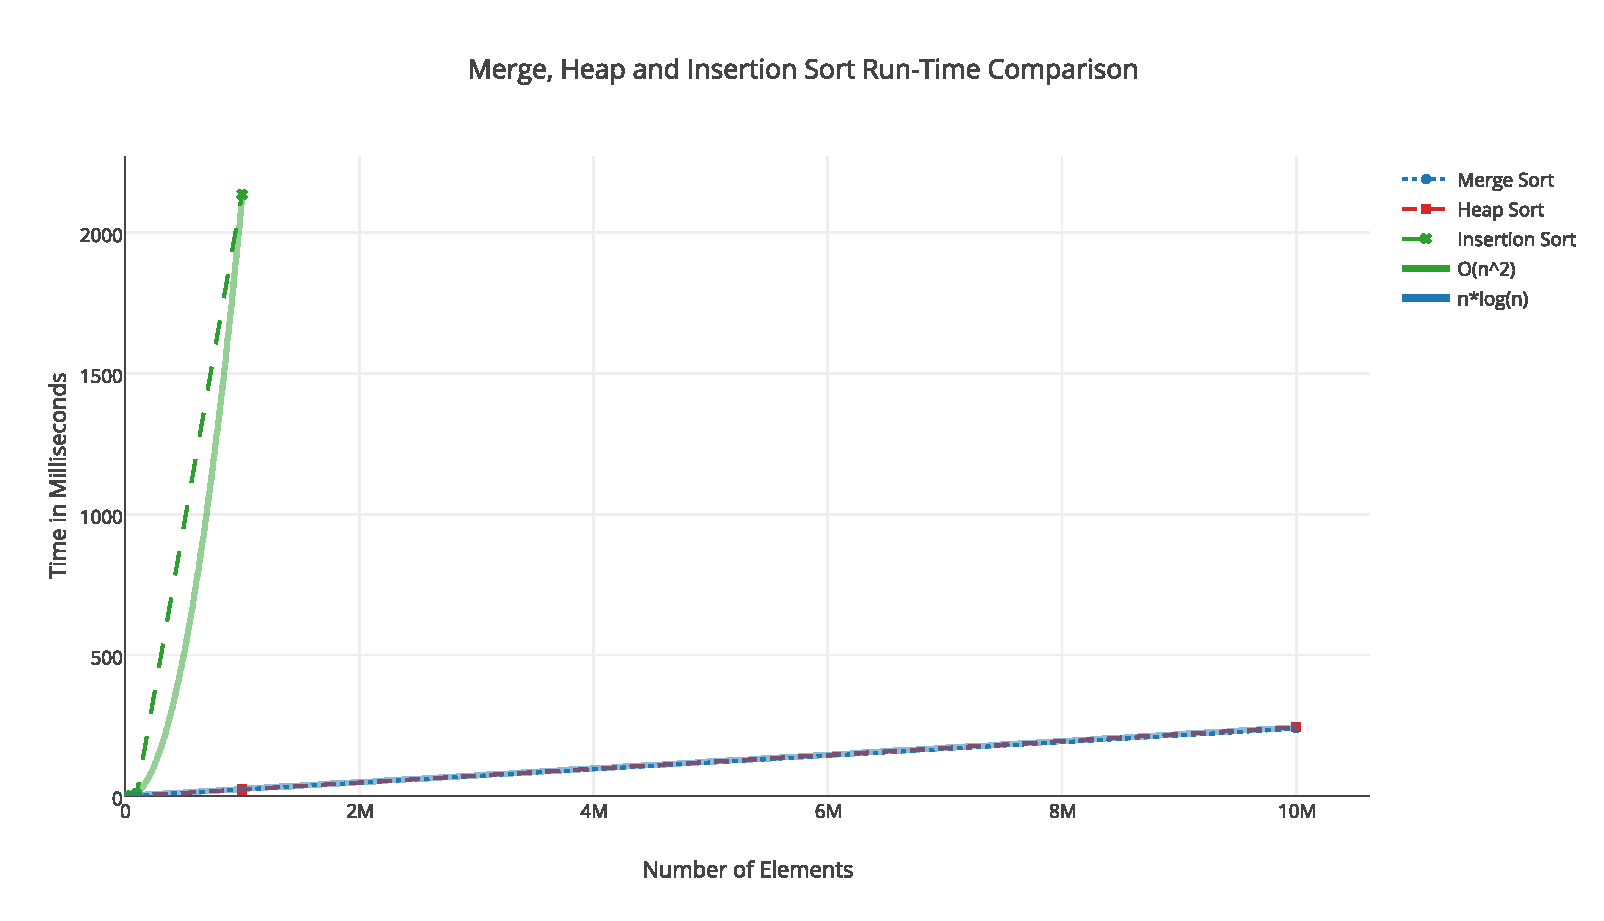
\includegraphics[scale=.70]{test-results.pdf}
\end{center}
\captionof{figure}{Merge, Heap and Insertion Sort Run-Time Comparison}
\label{fig:comparisonfig}
\end{figure}

The expected growth of insertion sort as the number of elements (n) grows large can be represented as $ \theta(n^2) $ where $ \theta() $ represents the asymptotically tightly bound running time. \cite{textbook} At $n_0$ the algorithm took 0.0003 milliseconds to complete. At $n_1$ the algorithm also took 0.0003 milliseconds to complete. For both these values of $n$, the algorithm runs at $ \theta(1) $, which is a constant value because the algorithm completes before a loop is run. As $n$ grows larger the time to complete the experimental data correlates quite accurately with the expected growth. For $n_{1*10^6} $ the data matches up perfectly. This is to be expected, because as n grows larger the constants and lower orders of the actual running time of the insertion sort start to affect the running time less and less as the highest order of $n^2$ is so large. It is expected for lower values of n to not correlate well with $ \theta(n^2) $ because the system running the algorithm may be executing superfolous commands such as checking for system. For the data graphed above (see Fig. 1) this was in fact the case. To aid this issue, averages of 10 trails were taken and used in Figure 1.

The expected growth of merge sort as the number of elements (n) grows large can be represented as $ \theta(n*\lg(n)) $. At $n_0$ the sort took 0.0002 milliseconds to complete, however, at $n_1$ the algorithm took 0.0001 milliseconds to complete. The discrepency can be attributed to superfolous commands being executed by the system. As $n$ grows larger the time to complete correlates with the expected running time. It is expected for lower values of $n$ to not correlate as nicely with the expected running time because the system constant will have a larger impact on the smaller values of $n$. It is important to note that merge sort ran much faster than insertion sort at large values of n such as $n_{1*10^6} $ and was able to process $n_{1*10^7} $ where insertion sort crashed the system. The best case running time for this implementation of merge sort is $ \theta(1) $ and is elicited only when $ n <= 1 $ because if $n <= 1$ the array is vacuously sorted and can be returned immediately without executing any loop, and run at a constant time.

Heap sort is very similar to merge sort in that its expected running time is $ \theta(n*\lg(n)) $. At lower values of $n$ heap sort ran marginally quicker than merge sort, however, as $n$ grew larger merge sort began to run marginally faster than heap sort. This difference is neglagable because of superfolous commands being executed by the system and other running processes. For all intensive purposes merge sort and heap sort have the same run time and the major difference between the two is the system constant. For $n_0$ heap sort completed in 0.0002 milliseconds and for $n_1$ heap sort completed in 0.0003 milliseconds. In both merge sort and insertion sort the sort completes before any loop is executed if $n <= 1$ however in this implementation of heap sort the algorithm runs through the entire sort. We can tell from this that the constant time is 0.0002 milliseconds, which correlates nicely with both merge and insertion sort. $ \theta(n*\lg(n)) $ is the both the best and worst case run-time for heap sort.
%% END EXPERIMENTAL ANALYSIS

%% BEGIN CONCLUSION
\section{Conclusions}
With a running time of $ \theta(n*\lg(n)) $ both heap sort and merge sort perform much faster than insertion sort at a running time of $ \theta(n^2) $, especially when $n$ grows large. While faster comptuers will be able to execute insertion sort faster, as $n$ grows large, even on a slower machine, both merge sort and heap sort will perform faster. Because it is easier to setup and maintain, insertion sort is a good choice when dealing with small sets of data that don't go beyond $n_{1*10^5}$, however, if data is expected to grow larger than that, either heap or merge sort is the best choice.
%% END CONCLUSION

\newpage

%% BEGIN REFERENCES
%%\section*{References}

\nocite{*}
\bibliographystyle{IEEEtran}
\bibliography{bib}

%% END REFERENCES

\newpage

%% BEGIN APPENDIX
\section*{Appendix}
\lstinputlisting[caption=Driver,
label={Driver.java},
breaklines=true,
]{Code/Driver.java}
\lstinputlisting[caption=Debug,
label={Debug.java},
breaklines=true,
]{Code/Debug.java}
\lstinputlisting[caption=DummyData,
label={DummyData.java},
breaklines=true,
]{Code/DummyData.java}

The class Stopwatch has not been altered from its original form.
\newline
\lstinputlisting[caption=Stopwatch,
label={Stopwatch},
breaklines=true,
]{Code/Stopwatch.java}
\lstinputlisting[caption=Sort,
label={Sort.java},
breaklines=true,
]{Code/Sort.java}
%% END APPENDIX

%% END DOCUMENT
\end{document}
